\documentclass{article}
\usepackage{amsmath, amssymb, mdwlist, graphicx, hyperref}
\usepackage{listings,color}
\usepackage{wrapfig}
\usepackage[usenames,dvipsnames]{xcolor}
\definecolor{gray}{rgb}{0.97,0.97,0.97}
\lstset{%
language=C,%
%backgroundcolor=\color{gray},
emph={putpixel},
emphstyle=\bf,
tabsize=4,
framesep=5pt,
mathescape=true,
xleftmargin=0.1cm,
xrightmargin=0.1cm,
frame=lines,
%basicstyle=\ttfamily,
%keywordstyle=\color{Blue},
%commentstyle=\color{OliveGreen},
%stringstyle=\color{MidnightBlue},
columns=flexible,
%showstringspaces=false
}

\newcommand{\mpar}[1]{\marginpar{\textit{#1}}}
\newcommand{\norm}[1]{\Vert #1 \Vert}
\DeclareMathOperator{\argmax}{argmax}
\DeclareMathOperator{\argmin}{argmin}
\newenvironment{solution}{\paragraph{Solution.}$\,$ }{\vskip 3mm\hrule}
\newenvironment{exercise}[2]{\paragraph{Exercise #1 (#2pt).} }{
\medskip}
\newcommand{\bbR}{\mathbb{R}}
\newcommand{\bw}{\mathbf{w}}
\newcommand{\bx}{\mathbf{x}}
\newcommand{\bd}{\mathbf{d}}
\newcommand{\bb}{\mathbf{b}}
\newcommand{\by}{\mathbf{y}}
\newcommand{\bzero}{\mathbf{0}}
\newcommand{\bz}{\mathbf{z}}
\newcommand{\bSigma}{\mathbf{\Sigma}}
\newcommand{\bp}{\mathbf{p}}
\newcommand{\bP}{\mathbf{P}}
\newcommand{\bm}{\mathbf{m}}
\newcommand{\bc}{\mathbf{c}}
\newcommand{\bM}{\mathbf{M}}
\newcommand{\bV}{\mathbf{V}}
\newcommand{\bK}{\mathbf{K}}
\newcommand{\bD}{\mathbf{D}}
\newcommand{\bA}{\mathbf{A}}
\newcommand{\bX}{\mathbf{X}}
\newcommand{\bY}{\mathbf{Y}}
\newcommand{\bR}{\mathbf{R}}
\newcommand{\bI}{\mathbf{I}}
\newcommand{\bS}{\mathbf{S}}
\newcommand{\bT}{\mathbf{T}}
\newcommand{\balpha}{\boldsymbol{\alpha}}
\newcommand{\pt}[2]{\left(\begin{array}{c}#1\\#2\end{array}\right)}

\begin{document}
\title{MTAT.03.015 Computer Graphics (Fall 2013)\\
Exercise session VIII: Textures}
\author{Konstantin Tretyakov, Ilya Kuzovkin}
\date{October 28, 2013}
\maketitle

Today we shall study the basics of OpenGL texture mapping. As usual, the code base is provided in \texttt{practice08.zip} archive on the course website or via the course github page. Download, unpack and open it. You will need to submit your solution as a zipped archive file.

\section{Basic Texture Mapping}
Open the project \verb#1_Flag# and study the code in \verb#flag.cpp#. The application shows a waving mesh. Your task is to configure and apply a ``flag'' texture to the mesh. The texture image is already loaded for you by calling the helper function \texttt{load\textunderscore texture} near the end of the \texttt{main} function. The global variable \texttt{textureHandle} represents the handle to this loaded texture.

\begin{exercise}{1}{0.5}
Add code to the \texttt{display} function that will add texture to the flag.
\begin{enumerate}
\item Enable texture mapping using \texttt{glEnable}.
\item Bind the texture into OpenGL context using \texttt{glBindTexture}.
\item Configure texture filtering parameters \verb#GL_TEXTURE_MIN_FILTER# and\\ \verb#GL_TEXTURE_MAG_FILTER#. Set them to the quality-wise best options.
\item Now we need to specify texture coordinates for each vertex of the mesh. For that we could go and change the \verb#draw_mesh# function, but this is quite unwieldy. Instead we shall rely on automatic texture coordinate generation. Enable it using \verb#glEnable(GL_TEXTURE_GEN_S)#,\\ \verb#glEnable(GL_TEXTURE_GEN_T)#.
\item At this point you should be able to see the texture being applied to the mesh. However, the texture coordinates are not computed in the way that we would like to. The default texture coordinate generation mode is \verb#GL_EYE_LINEAR#, which means that currently each vertex with camera-space position $(x, y, z)$ gets assigned texture coordinate $(x, y)$. As a result it seems that the texture is somehow fixed to the viewer rather than the object.

What we would like to do instead is to generate texture coordinates from the \emph{object-space} vertex positions, i.e. the vertex coordinates \emph{before} the model-view matrix is applied to them. This mode is called \verb#GL_OBJECT_LINEAR#. Enable it for both $s$ and $t$ coordinates using \\
\verb#glTexGeni( ... , GL_TEXTURE_GEN_MODE, GL_OBJECT_LINEAR)#.

\item The result is much better, although still incorrect. Currently the texture generation method directly uses vertex $(x,y)$ coordinates as the texture $(s,t)$ coordinates. The mesh is created so that its corners are at $(-1, -1)$, $(-1, 1)$, $(1, -1)$ and $(1, 1)$ (check out the \verb#draw_mesh# function). Those same coordinates are used to access the texture, which leads to the texture being repeated four times. Repeating the texture is the default method of interpreting texture coordinates outside of the range [0, 1].

Fortunately, OpenGL lets us specify linear $(x,y,z,w) \to (s,t)$ mappings for texture coordinate generation. Namely, by calling
\begin{verbatim}
    glTexGenfv(GL_S, GL_OBJECT_PLANE, s_map);
    glTexGenfv(GL_T, GL_OBJECT_PLANE, t_map);
\end{verbatim}
where \verb#s_map# and \verb#t_map# are four-element float arrays, we indicate that texture coordinates must be computed as follows:
\begin{align*}
s &:= \text{s\textunderscore map[0]}x + \text{s\textunderscore map[1]}y + \text{s\textunderscore map[2]}z + \text{s\textunderscore map[3]}w,\\
t &:= \text{t\textunderscore map[0]}x + \text{t\textunderscore map[1]}y + \text{t\textunderscore map[2]}z + \text{t\textunderscore map[3]}w.
\end{align*}
What is left is provide \verb#s_map# and \verb#t_map# such that the corners of the mesh will be assigned texture coordinates $(0, 0)$, $(0, 1)$, $(1, 0)$ and $(1, 1)$ respectively\footnote{Hint: $s := (x+1)/2,\quad t := (y+1)/2$.}. This will stretch the texture once over the whole mesh. Doing this completes this exercise.
\end{enumerate}
\end{exercise}

\begin{exercise}{2}{0.5}
Shaders provide more flexibility in how texture mapping can be done, so let us practice using them. Uncomment the line 
\begin{verbatim}
    texture_shader.use();
\end{verbatim}
near the end of the \texttt{main} function. This will replace the OpenGL fixed pipeline with the \texttt{flag.vert.glsl} and \texttt{flag.frag.glsl} vertex and fragment shaders. Lighting and texture modulation is already implemented there: study the code to understand how it is done. Then perform two changes.
\begin{enumerate}
\item Firstly, as we switch to shaders, automatic texture coordinate generation that we just configured via \texttt{glTexGen} stops working. Instead, we are responsible for filling in the \verb#gl_TexCoord[0]# global variable for each vertex in the vertex shader. Fix \texttt{flag.vert.glsl} to generate correct texture coordinates.
\item Secondly, our current fragment shader simply multiplies together the texture color with lighting computation result\footnote{This corresponds to the setting \texttt{glTexEnvi(..., GL\textunderscore TEXTURE\textunderscore ENV\textunderscore MODE, GL\textunderscore MODULATE)}, which is used by default, check the manual for \texttt{glTexEnv} to see what other options are possible in the fixed pipeline.}. Configure it instead so that the texture color would be used within the lighting computation, providing the \emph{ambient} and \emph{diffuse} colors of the fragment (leave the specular color white as before).
\end{enumerate}

If implemented correctly, you should get a picture like the following:
\begin{center}
\includegraphics[width=0.8\textwidth]{flag.png}
\end{center}

Finally, try changing the \verb#GL_SRGB# parameter in the \verb#load_texture# call to \verb#GL_RGB# and observe how incorrect interpretation of texture colors leads to incorrectly bright results\footnote{You could now make colors dark again by disabling the final gamma correction step in the fragment shader. Indeed, this is what many beginners usually do: forget both to decode sRGB when reading textures and to encode to sRGB on the output. This is, however, incorrect. Avoid doing so if possible.}.
\end{exercise}

\newpage

\begin{exercise}{3*}{0.5}
\begin{wrapfigure}{r}{0.5\textwidth}
\includegraphics[width=0.5\textwidth]{spotlight.png}
\end{wrapfigure}
Some flashlights have a particular pattern to their spotlight -- there might be a brighter spot in the center, then a darker ring, followed by a brighter region again. One possible way to implement this is to specify the spotlight intensity function in a one-dimensional array of floats, pass this array to the shader as a \emph{one-dimensional texture} and sample from this texture in the lighting computation. 

More precisely, while the spotlight attenuation is currently performed in the shader as follows:
\begin{verbatim}
  attenuation *= pow(cosA, light.spotExponent);
\end{verbatim}
the updated version would be 
\begin{verbatim}
  attenuation *= texture1D(spotlightTexture, cosA).x;
\end{verbatim}
In this exercise you are asked to add this feature. Some hints to help you:
\begin{enumerate}
\item You will need to create a new texture handle using \texttt{glGenTextures}, bind it to \verb#GL_TEXTURE_1D# and load the data from a one-dimensional array. \item You do not need mipmaps\footnote{Unless you decide to use a huge array with highly varying values.}, but you have to set the appropriate filtering options.
\item In the shader you will need to define a uniform variable of type \texttt{sampler1D}.
\item Once you use more than one texture, you have to explicitly tell OpenGL which variables in the shader correspond to which textures. The following code might be helpful\footnote{See also: \url{http://www.opengl.org/wiki/Sampler_(GLSL)\#Binding_textures_to_samplers}}:
\begin{verbatim}
    texture_shader.uniform1i("flagImage", 0);
    texture_shader.uniform1i("spotlightTexture", 1);
    glActiveTexture(GL_TEXTURE0);
    glBindTexture(GL_TEXTURE_2D, textureHandle);
    glActiveTexture(GL_TEXTURE1);
    glBindTexture(GL_TEXTURE_1D, secondTextureHandle);
\end{verbatim}
\end{enumerate}
\end{exercise}

\newpage
\begin{exercise}{4*}{0.5}
Render a sphere with the ``earth'' texture mapped on it. You can use the image file \verb#data/earth_sphere.jpg#, which provides a \emph{spherical Mercator projection} of the Earth surface\footnote{\url{http://en.wikipedia.org/wiki/Mercator_projection}. Do not confuse \emph{spherical projections} with \emph{sphere mapping}, an environment mapping technique.}, or find something more detailed in the Internet. Use \texttt{glutSolidSphere} and generate appropriate texture coordinates in the vertex shader\footnote{A sphere can also be rendered as a \emph{parametric surface} using \texttt{gluSphere}. Parametric surfaces (to be discussed in further lectures) provide very straightforward ways of generating texture coordinates (\texttt{gluQuadricTexture}). In this exercise, however, use \texttt{glutSolidSphere} none the less.}.
\end{exercise}

\section{Refraction}

\begin{wrapfigure}{r}{0.4\textwidth}
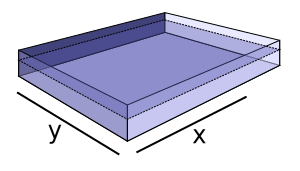
\includegraphics[width=0.4\textwidth]{rippletank.png}
\end{wrapfigure}
Suppose we are looking at a shallow tank with water. The bottom is covered with a picture and we are observing this picture from above through the thin layer of water. When the water is calm, we should be able to see picture in an undistorted form, however when there are ripples on the surface, the picture will be distorted due to refraction.

\begin{wrapfigure}{r}{0.4\textwidth}
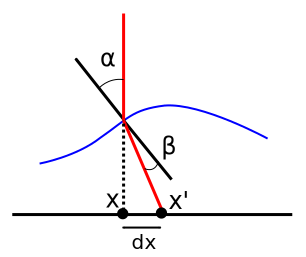
\includegraphics[width=0.4\textwidth]{refraction.png}
\end{wrapfigure}
The refraction process is illustrated on the figure to the right.

The red line corresponds to the ``ray of sight'' as it enters the water when the viewer is looking straight from above. If the water would be calm, the ray would continue straight on, hit the point $x$ on the bottom, and we would observe whatever is painted at that point on the bottom. 

However, as the water surface is not perpendicular to the ray, it is refracted and reaches the bottom of the tank at point $x'$, that is offset from $x$ by ${dx}$. 

The actual amount of displacement $dx$ can be computed exactly from the laws of refraction, however for the purposes of obtaining a visually convincing ``ripple'' effect a very simple approximation does a good job:
$$
dx \approx -k n_x,
$$
where $n_x$ is the corresponding coordinate of the surface normal vector and $k$ is some constant. Similarly, the displacement of the ray along the $y$ axis can be computed as
$$
dy \approx -k n_y.
$$

\begin{exercise}{5}{0.5}
Open the project \verb#2_Refract#. The project renders a flat grid mesh, and implements simple ``wavy'' mechanics for this mesh (move the mouse around to test it). A texture is applied to the mesh. However, currently the texture is mapped so that vertex with coordinate $(x, y, z)$ is assigned texture coordinates $(x, y)$. To simulate the rippling effect, apply the ideas described above and offset texture coordinates at each fragment as needed to imitate refraction. As a result you will observe convincing ripples. The picture below is a potential screenshot (it does not, though, provide a fair impression of the effect, as it does not show the dynamics of the process).
\begin{center}
\includegraphics[width=0.5\textwidth]{ripplecat.png}
\end{center}
Hint: in this exercise you need to change exactly one line in the vertex shader, one line in the fragment shader, and comment out one line in the \texttt{display} function.
\end{exercise}

\section{Reflection}
\begin{wrapfigure}{r}{0.4\textwidth}
\includegraphics[width=0.4\textwidth]{spheremap.jpg}
\end{wrapfigure}

A very similar idea can be used to render environmental reflections. Again, imagine the ``eyesight ray'' hitting a surface. If the surface is perfectly reflective, the ray will be reflected in some direction, that depends on the normal to this surface. 

Thus, let us precompute, for every possible direction of the normal, the color reflected by a surface with such normal. We shall store the precomputed values into a texture and use this texture whenever we need to render reflection at the fragments.

The simplest way to compute such a texture is to, literally, take a photo of a reflective ball (see image on the right). Now the pixel in the middle of the photo shows what should be reflected by a surface with its normal pointing straight into the viewer, the pixels at the top part of the ball show the reflections of surfaces with normals pointing up, etc.

This idea is called \emph{sphere mapping} and it is natively supported by OpenGL  without the need to write custom shaders. To use sphere mapping you simply have to load the appropriate texture and enable \verb#GL_SPHERE_MAP# texture coordinate generation mode (instead of \verb#GL_OBJECT_LINEAR# or \verb#GL_EYE_LINEAR# that you have seen before).

\begin{exercise}{6}{0.5}
Open the project \verb#3_SphereMap# and modify it to make the rotating teapot reflective.
\begin{enumerate}
\item Load the \verb#../data/spheremap.jpg# texture.
\item Enable texture coordinate generation.
\item Set the texture coordinate generation mode to \verb#GL_SPHERE_MAP#.
\item Do not forget to enable texturing.
\end{enumerate}
A total of just 7-9 lines needs to be added to \verb#sphere_map.cpp#. The result will look as shown below.
\begin{center}
\includegraphics[width=0.7\textwidth]{reflective_teapot.png}
\end{center}

\end{exercise}

\section{Normal mapping}
We have seen how textures can be used to store material parameters, intensity profiles, precomputed reflections and how refractions can be simulated by smart texture coordinate computation. Another popular application of textures is storing \emph{normals} to the surface at each point. This lets us imitate fine-grained detail on an otherwise flat polygon. The approach is called \emph{normal mapping}.

A particular subtype of normal mapping is \emph{bump mapping}. Here, the texture  represents a \emph{height map}, i.e. each texel stores a single number, which is the virtual ``height'' above the surface of a polygon. Normals at each point can be computed from the height map using discrete differentiation.

More specifically, consider a point $(x,y,0)$ of a polygon that lies in the $z=0$ plane. Let $t(x,y)$ denote the texture value at this point.

The normal to the height map at point $(x, y)$ can be computed as:
$$
\mathbf{n} = \text{normalize}\left(t(x-\varepsilon, y) - t(x, y), t(x, y-\varepsilon) - t(x, y), 1\right),
$$
where $\varepsilon$ is some small value (typically $\varepsilon = 1/n$, where $n$ is the height or width of the image in pixels). If we use the height-map normal in our lighting computations, the surface will seem to have a relief on it.

\begin{exercise}{7}{1}
Open the project \verb#4_BumpMap#. Your task is to modify the fragment shader in this project to implement bump-mapping as explained above. The result you might expect to get is shown below\footnote{If you follow the equations exactly as written, your relief won't be as sharp as the one shown here. You are free to rescale the heightmap to achieve the sharpness you like best.}.
\begin{center}
\includegraphics[width=0.8\textwidth]{bumpmap.png}
\end{center}
\end{exercise}

\begin{exercise}{8*}{0.5}
Continue Exercise 4: add a bump-map texture to the Earth (in addition to the usual color mapping), so that one could see the relief of mountains and oceans.
\end{exercise}


\end{document}
